\documentclass[00_complete]{subfiles}

%\documentclass[12pt]{report}
\usepackage[utf8]{inputenc}
\usepackage{amsmath,amssymb,amsthm,gensymb,parskip,graphicx,footmisc,csquotes,enumerate,datetime2}
\usepackage[]{libertinus}
\usepackage[breaklinks]{hyperref}
\hypersetup{
  pdfauthor={Moshe Krumbein},
  colorlinks=true,
  linkcolor={black},
  filecolor={black},
  citecolor={black}, %blue
  urlcolor={black}, %blue
}
\usepackage[top=30mm,bottom=30mm,left=30mm,right=30mm]{geometry}
%\setlength{\emergencystretch}{2em} % prevent overfull lines
\providecommand{\tightlist}{%
\setlength{\itemsep}{0pt}\setlength{\parskip}{0pt}}

\renewcommand\qedsymbol{$\blacksquare$}

\theoremstyle{definition}
\newtheorem*{definition}{Definition}
\newtheorem*{theorem}{Theorem}
\newtheorem*{axiom}{Axiom}
\newtheorem*{lemma}{Lemma}

\theoremstyle{remark}
\newtheorem*{note}{Note}
\newtheorem*{symbols}{Symbol}
\newtheorem{example}{Example}[section]
\newtheorem*{claim}{Claim}
\newtheorem*{conclusion}{Conclusion}
\newtheorem*{reminder}{Reminder}

\usepackage{fancyhdr}
\usepackage[italicdiff]{physics}
\MakeOuterQuote{"}

\renewcommand{\chaptermark}[1]{\markboth{#1}{}}

\pagestyle{fancy}

\setlength{\headheight}{14.5pt}
\addtolength{\topmargin}{-2.5pt}

\fancyhf{}
\rhead{Moshe Krumbein}
\lhead{\chaptermark}
\cfoot{\thepage}
\fancyhead[R]{\chaptername~\thechapter}
\fancyhead[L]{\mbox{\leftmark}}

\usepackage[Rejne]{fncychap}
\usepackage{titling}

\makeatletter
\renewcommand{\@chapapp}{\vspace*{-100pt}\huge\thetitle}
\makeatother

\makeatletter
\newcommand{\subtitle}[1]{%
  {\center\vspace*{-60pt}%
  \linespread{1.1}\Large\scshape#1%
  \par\nobreak\vspace*{35pt}}
}
\makeatother

\newcommand{\Chapter}[2]{
    \def\n{#2}
    \setcounter{chapter}{\the\numexpr\n-1}
    \chapter{#1}
    \subtitle{\theauthor~- \thedate}
}

\DeclareMathOperator{\Ima}{Im}
\DeclareMathOperator{\Id}{Id}
\DeclareMathOperator{\cis}{cis}

\newcommand{\Mod}[1]{\ (\mathrm{mod}\ #1)}
\newcommand{\st}[0]{\;\mathrm{s.t.}\;}

\title{Discrete Mathematics}
\author{Moshe Krumbein}
\date{Fall 2021}

\begin{document}
\Chapter{The Inclusion–Exclusion Principle}{7}

\section{Summation Principle}

\begin{theorem}
    If $A_1,\dots,A_n$ are \emph{pairwise disjointed}, then:
    $$\left|\bigcup_{i=1}^n\right| = \sum_{i=1}^{n}|A_i|$$
    However, there are $\binom{n}{2}$ conditions to check:
    $$\forall a,j \in [n]: A_i \cap A_j = \emptyset$$
\end{theorem}

\subsubsection{In General}

$$
\begin{aligned}
    n=2:& \quad|A \cup B| = |A| + |B| - |A \cap B| \\
    n=3:& \quad|A \cup B \cup C| = |A| + |B| + |C| - |A \cap B| - |A \cap C| - |B \cap
C| \\&+ |A \cap B \cap C|
\end{aligned}$$

\begin{figure}[ht]
  \centering
    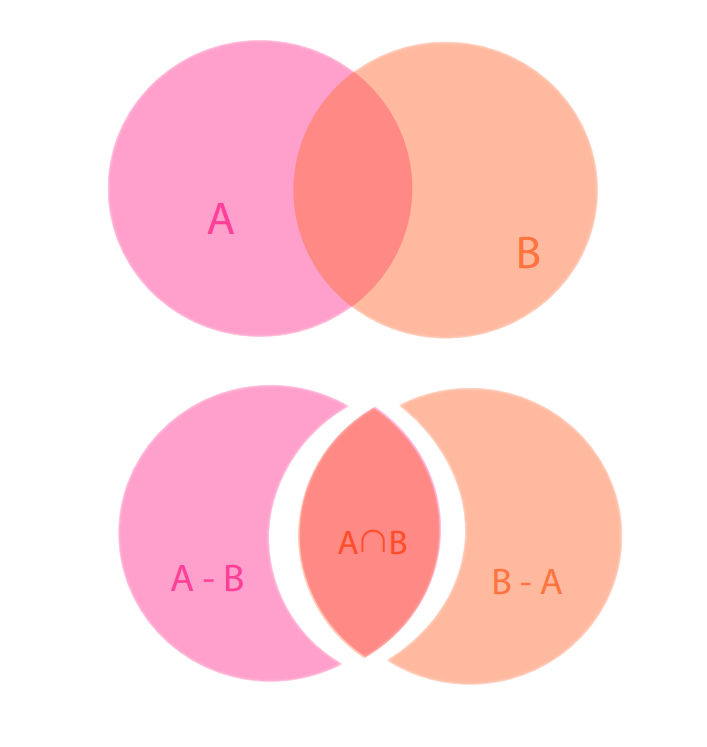
\includegraphics[width=0.25\textwidth]{w7_venn1}
    \caption{Visualization of $|A \cup B| = |A| + |B| - |A \cap B|$}
\end{figure}

\begin{symbols}
    $x$ is a finite set, and $A_1,\dots A_n$ are subsets of $x$.

    We symbolize $N=\{1,2,\dots,n\}$ for all $\emptyset \neq k \subseteq N$.
    $$A(k) = \bigcap_{i \in k}A_i$$
    \emph{For example}:
    $$k = \{1,4,5,8\} \implies A(k) = A_1 \cap A_4 \cap A_5 \cap A_8$$
\end{symbols}

\begin{theorem}[Inclusion-Exclusion Formula]
    $$\begin{gathered}
        |\bigcup_{i=1}^nA_i| = \underbrace{|A_1|+|A_2|+\dots+|A_n|}_{\binom{n}{1}}
    - \underbrace{|A_1\cap A_2|}_{\binom{n}{2}} \\\dots +(-1)^{n+1}|A_1\cap A_2
    \cap \dots \cap A_n|\\
    =\sum_{j=1}^{n}\sum_{\begin{subarray}{l} k \subseteq N \\ |k| =
    j\end{subarray}} (-1)^{j-1}|A(k)| \\
    = \sum_{k \subseteq N, k \neq \emptyset} (-1)^{|k|+1}|A(k)|
    \end{gathered}
    $$
    $$\boxed{\sum_{j=0}^n\sum_{\begin{subarray}{l}k \subseteq N \\ |k|= j\end{subarray}}
    (-1)^j|A(k)|}$$
\end{theorem}

\section{Review}

$X$ is a finite set. Sets $A_1, A_2, \dots, A_n \subseteq X$ (and are therefore
also finite).

We would like to find the size of $X \setminus (\bigcup_{i=0}^nA_i)$.

$N=\{1,2,\dots, n\} \forall k \subseteq N \neq \emptyset$:
$A(k)=\bigcap_{i\in k} A_i$, $A(\emptyset)=X$

Therefore:
$$
\begin{gathered}
\left|X \setminus (\bigcup_{i=0}^nA_i)\right|=|X|
-|A_1|-|A_2|-\dots-|A_n|
+\sum_{1\leq i < j \leq n}|A_i\cap A_j|\\
-\sum_{1 \leq i<j<k \leq n}|A_i\cap A_j \cap A_k|+\dots\\
=\sum_{j=0}^n\sum_{\begin{subarray}{1}k\subseteq
N\\|k|=j\end{subarray}}(-1)^j|A(k)|=
\sum_{k \subseteq N} (-1)^{|k|}|A(k)|
\end{gathered}
$$

\section{First Use}

\paragraph{Question:}

Given $S_n$ as permutations on $[n]$, and $\sigma \in S_n: 1\leq i \leq n$ is a
\emph{fixed point}, if $\sigma(i)=i$, our question is: how many permutations
$x$ exist that do not contain a \emph{fixed point}?

\paragraph{Solution:}
$$
\begin{gathered}
    x=S_n \quad |x|=n!\\
    \forall 1\leq i \leq n: A_i = \{\sigma \in S_n \mid \sigma(i)=i\}\\
    \bigcup_{i=1}^nA_i - \text{all of the permutations that contain at least one
    fixed point.}\\
    |A_i|=(n-1)! \quad 1 \leq i<j \leq n: |A_i \cap A_j|=(n-2)!\\
    \forall k \subseteq N: |k|=j: \quad |A(k)|=(n-j)!\\
    \left|X
    \setminus\bigcup_{j=0}^nA_i\right|=\sum_{j=0}^k\underbrace{\sum_{\begin{subarray}{1}k
    \subseteq
N\\|k|=j\end{subarray}}(-1)^j\underbrace{(n-j)!}_{|A(k)|}}_{\text{constant for
all $|k|=j$}} = \sum_{j=0}^{n}\binom{n}{j}(n-j)!(-1)^j \\
=n!\sum_{j=0}^n\frac{(-1)^j}{j!} \;\overrightarrow{\quad n \to \infty \quad}\;
n!\cdot\boxed{\frac{1}{e}}
\end{gathered}
$$

\section{Second Use}
Given finite sets $D,R: |D|=d, |R|=r$.
$$
    |A|=|\{f:D\to R \mid f \text{ is onto } (\Ima f=R) \}|=?
$$
If $d<r$, then $|A|=0$, and if $d=r$, then $|A|=r!$.

We're going to subtract from the total number of functions, all of the
functions that are not \emph{onto}.

\paragraph{Solution}
$$
\begin{gathered}
    X=\{f:D\to R\} \quad |X|=r^d\\
    \forall 1\leq i \leq r: A_i = \{f \in X \mid i \notin \Ima f\} \\
    \bigcup_{i=1}^rA_i - \text{All of the functions that are not onto.} \\
    A = X \setminus \bigcup_{i=1}^rA_i\\
\end{gathered}
$$
$$\begin{aligned}
    \forall 1 \leq i \leq r \quad &|A_i|&=(r-1)^d \\
    \forall 1 \leq i<j \leq r \quad &|A_i\cup A_j|&=(r-2)^d \\
    \forall k \subseteq R, |k|=j \quad &|A(k)|&=(r-j)^d
\end{aligned}$$
$$
\begin{gathered}
    \left|X \setminus \bigcup_{i=1}^rA_i\right| =
    \sum_{j=0}^{r}\sum_{\begin{subarray}{c}k \subseteq \{1,\dots
    r\}\\|k|=j\end{subarray}}(-1)^j|A(k)| =
    \sum_{j=0}^{r}\binom{r}{j}(-1)^j(r-j)^d
\end{gathered}
$$

\section{Third Use}

\begin{claim}
    For all $n \in \mathbb{N}$ there exists a factorization to primes, in
    other words primes $p_1,\dots,p_m$, $S_1,\dots,S_m\in \mathbb{N}$, such
    that:
    $$n=p_1^{S_1}p_2^{S_2}\dots p_n^{S_n}$$
\end{claim}

\begin{definition}
    For $m,n \in \mathbb{N}$, we say that $m$ and $n$ are \emph{relatively
    prime} or \emph{coprime} if:
    $$\gcd(m,n)=\max\{k \in \mathbb{N}\mid k|m, k|n\} = 1$$
    In other words, they do not share any prime factors.
\end{definition}

\begin{claim}
   If $k,n \in \mathbb{N}$, then the number of terms between $1$ and $n$ that
   divides $k$ is $\lfloor\frac{n}{k}\rfloor$.

   In other words, $|\{1 \leq i \leq n \mid i \in \mathbb{N},
   k|i\}|=\lfloor\frac{n}{k}\rfloor$
\end{claim}

\paragraph{Explanation}

If we symbolize $l=\lfloor\frac{n}{k}\rfloor$, $l$ is the largest integer such
that $l \leq \frac{n}{k}$.
$$
\begin{gathered}
    A=\{k,2k,3k,\dots,lk\} \quad lk \leq \frac{n}{k}k=n \\
    |A|=l=\left\lfloor\frac{n}{k}\right\rfloor
\end{gathered}
$$

\paragraph{Question}

Given $n \in \mathbb{N}$ how many numbers $\{1,\dots,n\}$ are \emph{coprime} to
$n$?

\begin{definition}[Euler's totient function]
    $$\varphi(n) = |\{x \in \mathbb{N} \mid x \leq n;
        x,n \text{ are \emph{coprime}}\}|
    $$
\begin{example}
    $$\varphi(12)=|\{1,5,7,11\}|=4$$
    If $p$ is prime, then $\varphi(p)=|\{1,2,3,\dots,p-1\}|=p-1$.
\end{example}
\end{definition}
\begin{theorem}[Euler's totient function]
    For $n \in \mathbb{N}$ if:
    $$n=p_1^{s_1}p_2^{s_2}\dots p_t^{s_t}$$
    then:
    $$\varphi(n)=n\prod_{i=1}^t\left(1-\frac{1}{p_i}\right)$$
    \begin{example}
        $$\varphi(12)=12\cdot\left(1-\frac{1}{2}\right)\left(1-\frac{1}{3}\right)=4$$
    \end{example}
\end{theorem}
\begin{proof}
    First, we notice that if $m \in \mathbb{N}$ is not \emph{coprime} with $n$, then there
    exists some $1\leq i \leq t$ such that $p_i|m$.

    We define $x=[n]$.
    $$
    \begin{aligned}
        \forall i: 1 \leq i \leq n:
        \quad &A_i = \{x \in [n] \mid p_i|x \} \quad&|A_i|=\frac{n}{p_i} \\
        1 \leq i<j\leq n:
        \quad &A_i\cap A_j = \{x \in [n] \mid p_i|x, p_j|x \}  \quad &|A_i \cap A_j| =\frac{n}{p_ip_j} \\
    \end{aligned}
    $$
    And in general:
    $$
    \begin{gathered}
        k \subseteq \{1,\dots,t\} \\
        A(k)=\bigcap_{i \in k}A_i = \{x \in [n] \mid \forall i \in k: p_i|x\}
        = \left\{x \in [n] \;\middle|\; \prod_{i \in k}p_i|x\right\} \\
        |A(k)| = \frac{n}{\prod_{i \in k}p_i}
    \end{gathered}
    $$
    Based on our definition:
    $$
    \begin{gathered}
        \varphi(n) = \left|X \setminus \bigcup_{i=1}^tA_i\right|
        = \underbrace{n}_{|X|}-\sum_{i=1}^{t}\frac{n}{p_i}+\sum_{1\leq i<j\leq
        n}\frac{n}{p_ip_j}-\sum_{1\leq i<j<j\leq n}\frac{n}{p_ip_jp_k}+\dots\\
        +(-1)^j\sum_{\begin{subarray}{c}k \subseteq
        \{1,\dots,t\}\\|k|=j\end{subarray}}\frac{n}{\prod_{i \in k}p_i}\\
        =n\sum_{j=0}^{n}(-1)^j\sum_{\begin{subarray}{c}k \subseteq
        \{1,\dots,t\}\\|k|=j\end{subarray}}\frac{1}{\prod_{i \in k}p_i}
    \end{gathered}
    $$
    With a little algebraic manipulation, we can see that our conclusion is
    indeed equal to:
    $$n\prod_{i=1}^t\left(1-\frac{1}{p_i}\right)$$
\end{proof}
\end{document}
